\chapter{Aspectos Conceituais}
    \section{Scrum} %% TODO: Luiz 
    Scrum\cite{essentialscrum} é um método de desenvolvimento de produtos e serviços. Esse método teve concepção em 1986, Em uma publicação\cite{scrumorigin} de Takeuchi e Nonaka, que descrevem bons resultados obtidos em grandes empresas usando a metodologia.
    
    O início da execução do \textit{Scrum} é criar uma lista priorizada de \textit{features} (funcionalidades) e outras capacidades necessárias pra se desenvolver um produto com sucesso, chamada de \textbf{backlog}. A implementação sempre tem que seguir a ordem de prioridade atribuída a cada \textit{feature}, sendo sempre executado primeiro o que for mais prioritário.
    
    O trabalho é feito em \textit{Sprints}: iterações de tempo curto e limitado (em geral de 1 ou 2 semanas). A execução é feita por uma equipe multi-funcional e auto-contida, com desenvolvedores, arquitetos, engenheiros, \textit{designers}, etc, de modo que ao final da \textit{Sprint} obtém-se uma parte do produto que traz algum valor de negócio.
    
    No final da \textit{Sprint}, a equipe revisa o que foi feito com os \textit{stakeholders} e ajusta a priorização de acordo com o \textit{feedback}. O ciclo recomeça com uma reunião de planejamento para a próxima iteração.
    
    \begin{figure}[htb]
		\caption{\label{fig:scrum} Framework do scrum}
		\begin{center}
		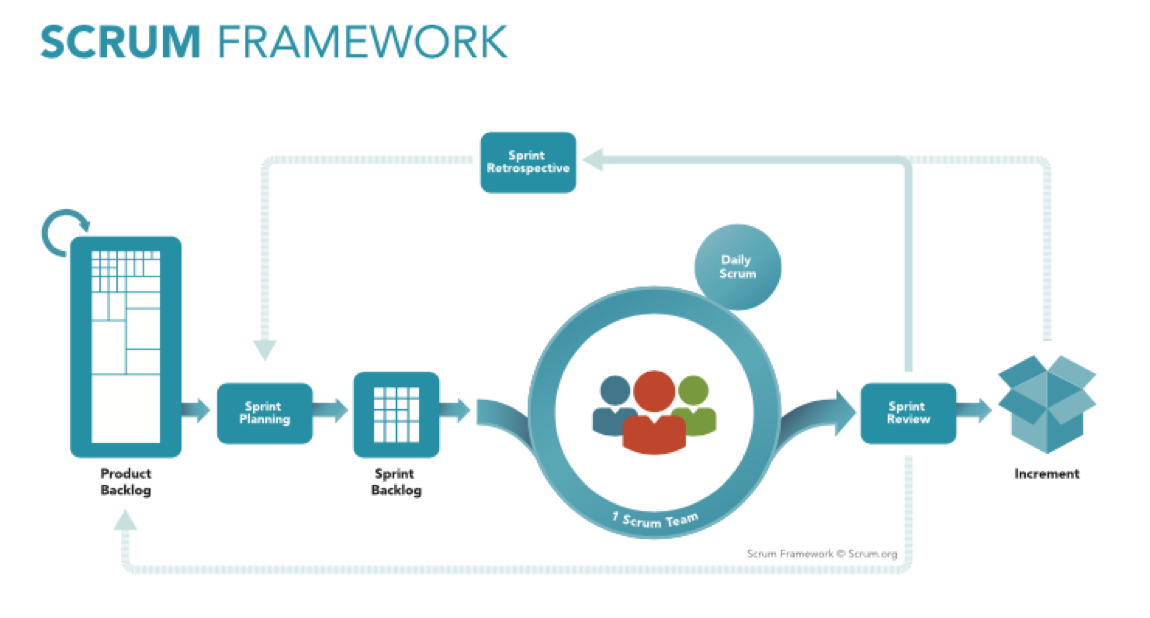
\includegraphics[width=\textwidth,keepaspectratio]{pictures/ScrumFrameworkTest.png}
		\end{center}
		\legend{Fonte: https://www.scrum.org/resources/what-is-scrum}
	\end{figure}

	\section{Cloud Computing}
	Computação em Nuvem (do Inglês \textit{Cloud Computing}) é segundo a NIST \footnote{National Institute of Standards and Technology, https://www.nist.gov/} um modelo para prover um acesso de rede a um grupo compartilhado (\textit{shared pool}) de recursos computacionais (recursos como capacidade de rede, servidores, armazenamento, aplicações e serviços) de forma ubíqua, prática e sob demanda.

Tal acesso deve ser rapidamente provisionado e lançado com o mínimo de gerenciamento e interação com o provedor de serviços por parte da aplicação.

O modelo de computação em nuvem deve possuir algumas características básicas, que estão descritas na seção seguinte.

\subsection{Características básicas de Cloud Computing}

A NIST define 5 características essenciais do modelo de Cloud Computing:
\begin{itemize}
	\item Serviço sob demanda: Um consumidor pode provisionar unilateralmente capacidades computacionais, como tempo de servidor e armazenamento de rede, conforme for necessário, sem qualquer interação humana com o provedor de serviço;
	\item Agrupamento de recursos: Os recursos de computação do provedor são agrupados para atender a vários consumidores usando um modelo "multi inquilino", com diferentes recursos físicos e virtuais dinamicamente atribuídos e reatribuídos de acordo com a demanda do consumidor. Existe uma sensação de independência de localização pois o cliente geralmente não tem controle ou conhecimento sobre a localização exata dos recursos fornecidos, mas pode ser capaz de especificar a localização em um nível de abstração (por exemplo, país, estado ou datacenter). Exemplos de recursos incluem armazenamento, processamento, memória e largura de banda de rede.
	\item Amplo acesso à rede: Os recursos estão disponíveis na rede e são acessados por meio de mecanismos que promovam o uso por plataformas heterogêneas por clientes em diversos dispositivos (por exemplo, telefones celulares, tablets, laptops e estações de trabalho). Esta característica promove o conceito de computação ubíqua, isto é, em toda parte, onipresente.
	\item Elasticidade rápida: Os recursos podem ser provisionados e liberados elasticamente, em alguns casos automaticamente, proporcionando uma escalabilidade crescente ou descrescente conforme a demanda. Os recursos disponíveis normalmente aparentam ser ilimitados para o consumidor, podendo ser requisitidados em qualquer quantidade e a qualquer momento.
	\item Serviço mensurável: Os sistemas em nuvem controlam e otimizam automaticamente o uso de recursos, aproveitando-se de uma capacidade de medição em um nível de abstração apropriado ao tipo de serviço (por exemplo, armazenamento, processamento, largura de banda e contas de usuário ativas). O uso de recursos pode ser monitorado, controlado e reportado, gerando transparência tanto para o fornecedor e consumidor do serviço utilizado.
\end{itemize}

\subsection{Modelos para Cloud Computing}

Este capítulo introduz brevemente os modelos de serviço de cloud computing que podem ser adotados por um provedor e os modelos de \textit{deployment}, nas secções seguintes.

\subsection{Modelos de serviços}

A teoria por trás dos serviços de computação em nuvem abrange três elementos principais: software, plataforma e infraestrutura. Temos os seguintes modelos de serviço:

\begin{itemize}
  \item \textbf{SaaS, Software as a Service} ("Software como um serviço") 

  Neste modelo é oferecido ao consumidor o uso de aplicações de um provedor que rodam sobre uma infraestrutura em nuvem. Estas aplicações são acessíveis a partir de vários dispositivos clientes por meio de uma interface simples, como um navegador da web, ou uma interface de por meio de um programa (mobile ou desktop). 

  O consumidor não gerencia ou controla a infraestrutura de nuvem por trás da aplicação, incluindo rede, servidores, sistemas operacionais, armazenamento ou capacidade da aplicação individual. São disponibilizadas apenas configurações do aplicativo específicas para aquele usuário individual.

  Alguns exemplos de SaaS são serviços de \textit{webmail}, \textit{streaming} de vídeos, conversão de arquivos e trabalho colaborativo com arquivos. Este modelo não será mais detalhado neste trabalho.

  \item \textbf{PaaS, Platform as a Service} ("Plataforma como um serviço") 

  A capacidade fornecida ao consumidor é de implantar na nuvem aplicações criadas por meio de linguagens de programação, bibliotecas, serviços e ferramentas suportadas pelo provedor. Tais aplicações podem ser criadas pelo próprio consumidor, ou consumidas por este.

  Assim como no modelo de SaaS, o consumidor geralmente não gerencia ou têm controle sobre a infraestrutura de nuvem por trás, incluindo rede, servidores, sistemas operacionais, ou armazenamento. Porém o consumidor as tem controle sobre os aplicativos implantados e possivelmente sobre definições de configuração para o ambiente de hospedagem do aplicativo.

  Como exemplos de provedores no mercado temos \textit{IBM Bluemix}, \textit{Heroku}, e \textit{Windows Azure Cloud}.

  \item \textbf{IaaS, Infrastructure as a Service} ("Infraestrutura como um serviço") 

  A capacidade oferecida ao consumidor é provisionar processamento, armazenamento, redes e outros recursos fundamentais de computação onde o consumidor é capaz de implantar e executar software arbitrário, incluindo-se sistemas e aplicações. O consumidor não gerencia nem controla a infraestrutura de nuvem por trás, mas tem controle sobre sistemas operacionais, armazenamento e aplicativos implantados. Possivelmente possui também um controle limitado de componentes de rede (por exemplo, firewalls de host). Geralmente acompanha serviços de máquinas virtualizadas.

  Alguns exemplos de provedores no mercado são \textit{Amazon Web Services}, \textit{Microsoft Azure}, \textit{Google Cloud} e \textit{VMware Cloud on AWS}. 
\end{itemize}

\subsection{Modelos de implantação}
Os modelos de implantação (\textit{deployment models}) a seguir delimitam as formas pos\-sí\-veis de tarifação dos serviços, as possíveis localizações da infraestrutura física e o público de escopo. São eles:

\begin{itemize}
  \item \textbf{Nuvem privada}: A infraestrutura de nuvem é disponibilizada para uso exclusivo por uma única organização, compreendendo vários consumidores (\textit{business units}). Pode ser propriedade e gerenciada pela própria organização, um terceiro ou alguma combinação de ambos, e pode existir dentro ou fora das instalações da organização.
  \item \textbf{Nuvem comunitária}: A infraestrutura em nuvem é de uso exclusivo por uma comunidade de consumidores de organizações que compartilham mesmos interesses (por exemplo, missão, requisitos de segurança, políticas e considerações de conformidade). Pode ser de propriedade e administrada por uma ou mais organizações da comunidade, um terceiro, ou alguma combinação de ambos, e pode existir dentro ou fora das instalações.
  \item \textbf{Nuvem pública}: A infraestrutura de nuvem é para o uso aberto pelo público em geral. Pode ser propriedade ou gerenciada por uma organização comercial, acadêmica ou governamental, ou alguma combinação destes. Existe dentro das instalações do provedor de nuvem.
  \item \textbf{Nuvem híbrida}: A infraestrutura de nuvem é uma composição de duas ou mais infraestruturas de nuvens distintas (privadas, comunitárias ou públicas) que permanecem como entidades únicas, mas unidas por tecnologia padronizada ou proprietária permitindo portabilidade de dados e aplicações (por exemplo, \textit{cloud bursting} para balanceamento de carga entre nuvens).
\end{itemize}

	\section{Programação Funcional}
	
	Como o próprio nome diz, a programação funcional surge de funções matemáticas, mais especificamente do cálculo lambda. Programação funcional é um paradigma de programação assim como Orientado a Objeto ou Imperativo. As características mais marcantes desse paradigma são a presença de imutabilidade de dados e estados, funções serem tratadas como valores como quaisquer outros tipos (inteiros, strings, etc...), transparência referencial e separação de efeitos colaterais.
	As linguagens de programação podem ser puramente funcionais, ou parcialmente, isso é, contém elementos desse paradigma porém não se limitam a ele, ou fazem pequenos desvios em prol da usabilidade.
	
	\section{Microsserviços}
	
	Microsserviços é um termo para designar uma arquitetura de software distribuída que possui um certo conjunto de características, como por exemplo o deploy independente. Em resumo é uma abordagem de desenvolvimento que que permite a criação de uma aplicação única através de um conjunto de pequenos serviços, de modo que cada um é responsável apenas por uma pequena parte do processo e durante sua execução eles se comunicam por meio de mecanismos leves, geralmente uma API e/ou mensageria (mas não se limitando a esses). Cada um dos serviços é focado em uma parte atômica da lógica de negócio e funcionam através de mecanismos de deploy independente e automatizado. Em contraste a esse tipo de arquitetura temos uma aplicação monolítica, que se caracteriza pela centralização da lógica e código em apenas um serviço de grande porte. \cite{microsservicos}
	
	\begin{figure}[htpb]
	    \caption{Microsserviços vs Monolitos}
	    \begin{center}
	        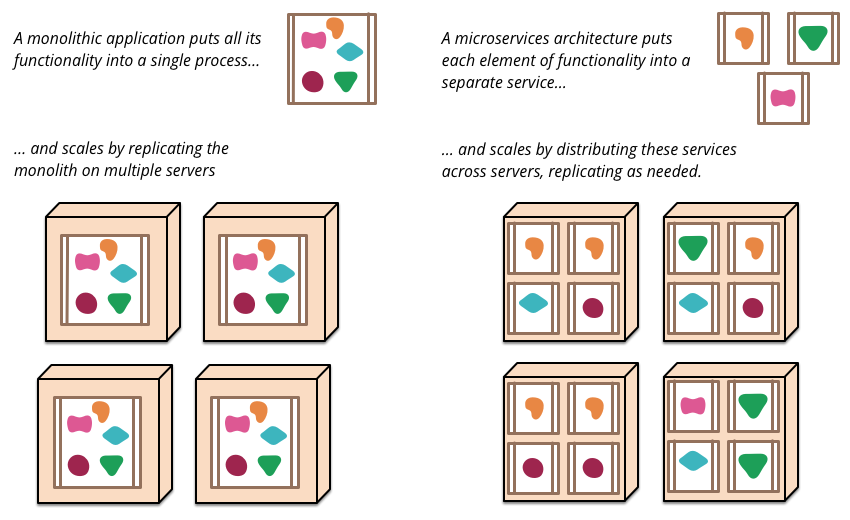
\includegraphics[scale=0.4]{pictures/sketch_microservices.png}
	    \end{center}
	    \label{fig:microsservicos_vs_monolito}
	    \legend{Fonte: https://martinfowler.com/articles/microservices/images/sketch.png}
	\end{figure}
	
	\section{HTTP} %% TODO: Paps
	Acrônimo de \textit{HyperText Transfer Protocol}. Protocolo usado pela \textit{Web}, define formato de mensagens trafegadas e formatação, dando também orientações semânticas via códigos\cite{httpcodes} de como os \textit{browsers} ou servidores devem reagir em resposta a diversos comandos.
	
	\section{Arquitetura Hexagonal}
	
	Também conhecida com Arquitetura de \textit{Ports and Adapters} é um modelo de arquitetura de software em camadas que presa pela separação entre domínio e lógica da aplicação com comunicação e interação com o mundo exterior. Esse modelo possui as seguintes camadas:
	
	\begin{itemize}
	    \item Port
	    \item Adapter
	    \item Controller/Application
	    \item Domain/Logic
	\end{itemize}
	
	Sendo as responsabilidades de cada camada as seguintes:
	
	\textbf{Ports}: São a camada responsável por realizar o interfaceamento com algum tipo de IO, seja HTTP, Mensageria, Banco de Dados, ou qualquer outro.
	
	\textbf{Adapters}: Camada responsável por realizar a adaptação e transformação entre dados de um modelo do domínio interno para uma representação a ser usada externamente para alguma porta.
	
	\textbf{Controller/Application}: Tem o papel de controlar a interação e chamadas entre as portas junto as funcionalidades do domínio da aplicação.
	
	\textbf{Domain/Logic}: Lógica e modelos internos e específico da aplicação, contém a lógica principal do serviço.
	
	\begin{figure}[htpb]
	    \caption{Diagrama de Arquitetura Hexagonal}
	    \begin{center}
	        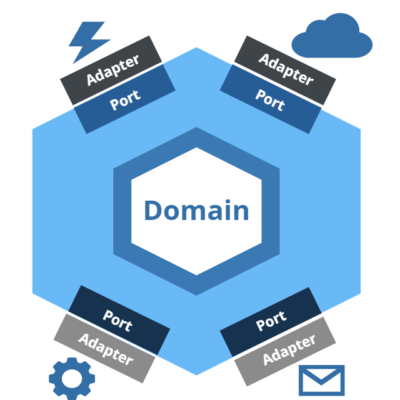
\includegraphics[scale=0.6]{pictures/hexagonal1.png}
	    \end{center}
	    \label{fig:hexagonal1}
	    \legend{Fonte: https://lmonkiewicz.com/wp-content/uploads/2017/04/hexagonal-e1491766585240.png}
	\end{figure}

	A grande possibilidade desse modelo é que ele permite que se tenham diversas portas e adaptadores diferentes para um mesmo domínio/lógica da aplicação, como o diagrama abaixo mostra.
	
	Essa arquitetura é muito interessante para microsserviços pois permite criar um desacoplamento de forma natural e da grandes possibilidades de meios de comunicação e interação dos serviços entre si.
	
	\section{Git}
	
	Git é um sistema de controle de versões distribuído amplamente utilizado em desenvolvimento de software. o Git se organiza através de repositórios que podem ser clonados e editados localmente pelo usuário e então sincronizados com um servidor remoto, publicando as alterações. Todo o histórico de alterações é mantido nesse processo sem perda de informações.
	Alguns conceitos importantes de serem destacados no funcionamento do Git para o melhor entendimento desse projeto são os seguintes:
	
	\textbf{Repositório}
	\newline
	Corresponde a um diretório de arquivos gerenciado pelo Git.
	
	\textbf{Commit}
	\newline
	É uma consolidação de um conjunto de alterações realizado no repositório Git. Representa um ponteiro para um estado específico (uma versão).
	
	\textbf{Branch}
	\newline
	Branch é um ponteiro movél que aponta para um determinado commit. Branches criam a ideia de uma árvore de caminhos em um repositório apontam sempre para o commit mais recente de uma bifurcação de mudanças.
	
	\textbf{HEAD}
	\newline
	HEAD é um ponteiro que aponta para para o branch ou commit atual que está em uso no repositório local.
	
	\textbf{FETCH\_HEAD}
	\newline
	Um ponteiro efêmero que aponta para a última referência buscada por um fetch.
	
	\textbf{Staging}
	\newline
	Área do Git onde as alterações que vão entrar no próximo commit ficam
	
	\begin{figure}[htbp]
		\caption{\label{fig_git1}Anatomia do Git}
		\begin{center}
		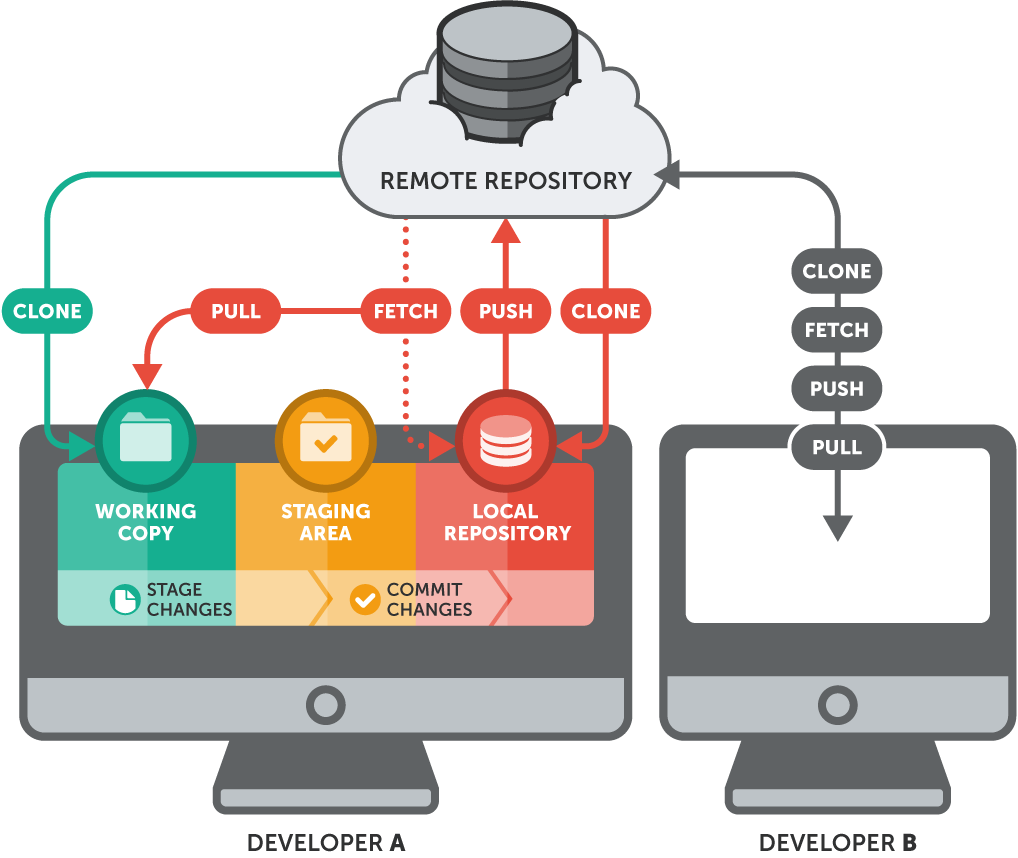
\includegraphics[scale=0.4]{pictures/git.png}
		\end{center}
		\legend{Fonte: \url{https://raw.githubusercontent.com/UnbDroid/AprendendoGithub/master/images/git.png}}
	\end{figure}
	
	Para realizar a sincronização entre repositórios locais e remotos o Git possibilita o uso de diversos protocolos de rede, temos entre eles principalmente: HTTP(S), FTP, rsync ou SSH.
	
	Durante o processo de uso do Git algumas ações são frequentemente utilizadas, e valem ser destacadas aqui, essas são:
	\begin{itemize}
    	\item \textbf{git init:} 
    	Inicia um repositório git vazio no diretório.
    	
    	\item \textbf{git clone:}
    	Cria um cópia de um repositório remoto localmente, acaba por fazer um download da estrutura remota para a maquina do usuário.
    	
    	\item \textbf{git fetch:}
	    Sincroniza o estado do repositório remoto com o local sem realizar alterações na \textit{working tree} do desenvolvedor. Baixa os dados existentes no repositório remote que não existem no computador do usuário.
	
    	\item \textbf{git checkout:}
    	Alinha o repositório local de acordo com a revisão ou branch especificado no comando.
    	
    	\item \textbf{git commit:}
    	O commit é o ato de criar um ponto no histórico do repositório contendo as mudanças que foram adicionas na área de staging.
    	
    	\item \textbf{git add:}
    	O comando \textit{add} é responsável por adicionar as mudanças especificadas na área de staging do git para serem comitadas em seguida.
    	
    	\item \textbf{git push:}
    	O push executa a ação de enviar os commits locais para o repositório remoto especificado.
    	
    	\item \textbf{git merge:}
    	Atualiza os arquivos na working tree para corresponderem ao especificado no comando. O merge também pode acabar atualizando o HEAD do branch atual.
    	
    	\item \textbf{git pull:}
    	Esse comando realiza a atualização do repositório local a partir das mudanças realizadas no repositório remoto. De forma geral ele acaba realizando um download dos commits mais recentes que estão presentes no remote. É uma combinação do git fetch com o git merge FETCH\_HEAD
	\end{itemize}
	\begin{figure}[htb]
		\caption{\label{fig_git2}Fluxo de trabalho em Git}
		\begin{center}
		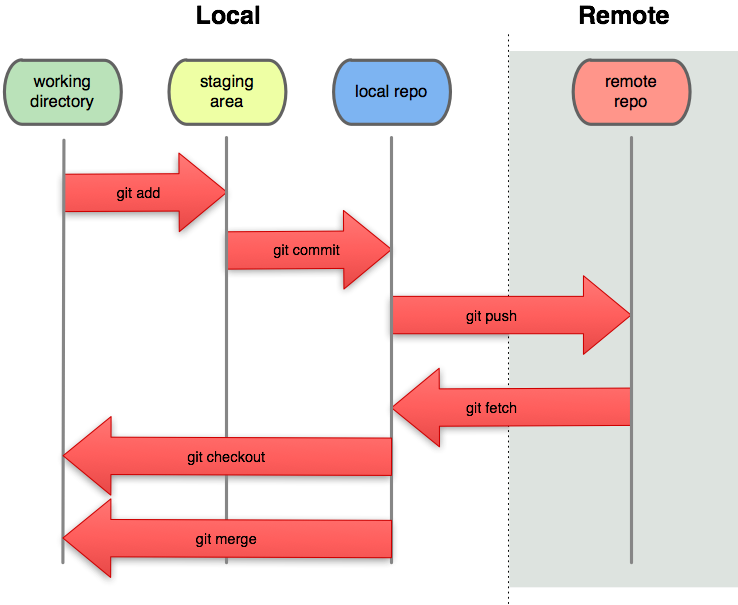
\includegraphics[scale=1]{pictures/GIT2.png}
		\end{center}
		\legend{Fonte: \url{https://kevintshoemaker.github.io/StatsChats/GIT2.png}}
	\end{figure}

	\section{Distributed Tracing}
	
	Distributed Tracing, ou Rastreamento Distribuído, é uma técnica utilizada em sistemas distribuídos para conseguir acompanhar algum fluxo que acaba por interagir com diversos serviços. Muito utilizado para ajudar desenvolvedor em sessões de depuração afim de entender qual caminho de código está sendo executado e com quais parâmetros em um sistema complexo e distribuído. Geralmente esse sistema se compõe de um broker central para onde as métricas e dados de tracing são enviados pelos serviços, e um conjunto de código que roda em todos os serviços, responsável por realizar a amostragem e enviar esses dados para o broker principal. Enquanto os brokers esperam receber mensagens representando eventos de entrada ou saída dos serviços através de um processo coletor, as bibliotecas se encarregam de enviar essa menagem e também propagar informações de rastreabilidade para as próximas interações com outros serviços. Podemos ver um digrama exemplificando a arquitetura de um Distributed Tracing nas figuras \ref{fig_tracing_concept} e \ref{fig_tracing_components}
	
	\begin{figure}[htb]
		\caption{\label{fig_tracing_concept}Anatomia de um Distributed Tracing}
		\begin{center}
		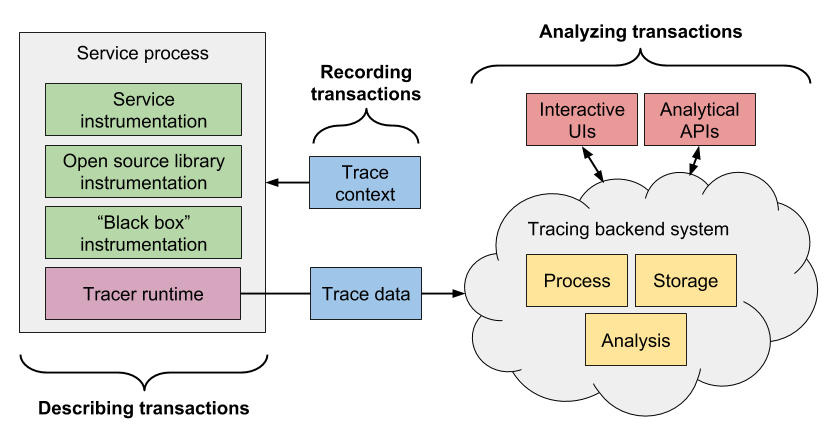
\includegraphics[scale=0.5]{pictures/tracing_concept.png}
		\end{center}
		\legend{Fonte: \url{https://cdn-images-1.medium.com/max/838/1*NuwuCvqZHLBJcJycRr1HTw.png}}
	\end{figure}
	
	\begin{figure}[htb]
		\caption{\label{fig_tracing_components}Componentes de um Distributed Tracing}
		\begin{center}
		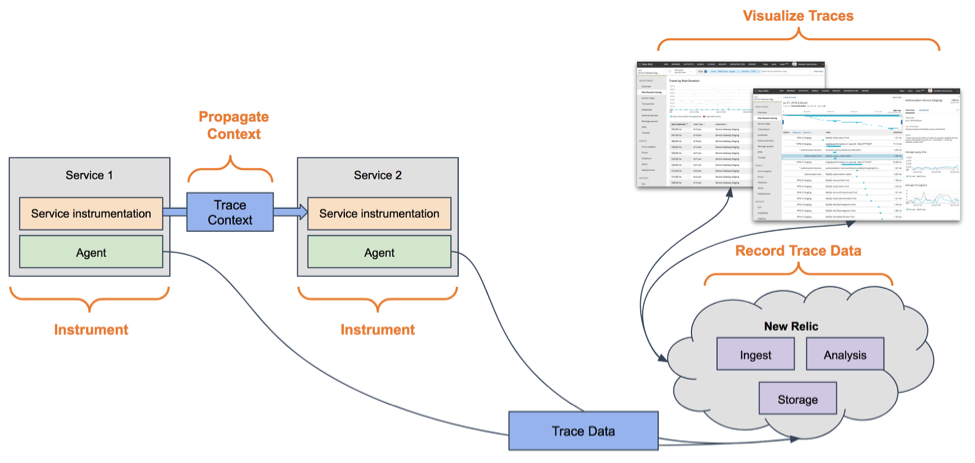
\includegraphics[scale=0.95]{pictures/distributed-tracing-components.png}
		\end{center}
		\legend{Fonte: \url{http://blog.newrelic.com/wp-content/uploads/Distributed-tracing-components.png}}
	\end{figure}
	
	Um dos primeiros Distributed Tracers que foi desenvolvido, foi o Dapper \cite{googledapper}, pela Google em meados de 2010. Com a abertura do código do Dapper outras empresas acabaram se interessando pelo projeto e funcionalidades e criaram suas próprias versões de tracers, entre eles alguns dos mais famosos: Zipkin\cite{zipkin}, pelo Twitter, e Jaeger\cite{jaegerarch}, pela Uber. Com o surgimento de novos tracers no mercado, a industria entrou em busca de um padrão para esse tipo de software, originando-se o OpenTracing\cite{opentracing}. OpenTracing é um padrão desenvolvido afim de definir normas e regras e padrões para implementação de Distributed Tracers. Nela são descritos estratégias para se realizar a identificação de informações gera mente importantes e o formato do tráfego de dados entre os serviços e os brokers.
	
	Grande parte do valor dos Distributed Tracing vem de suas ferramentas analíticas, que facilitam a vida do desenvolvedor e permitem com que ele faça análises de forma rápida e eficiente nos sistemas. Geralmente essas ferramentes vem junto com uma aplicação de Frontend que consegue exibir fluxos e montar gráficos. Entre eles o Flamegraph é muito utilizado para visualizarmos como a comunicação se aprofunda e se propaga na rede, uum exemplo de Flamegraph do Zipkin pode ser visto na figura \ref{fig_zipking_sample}. Outro tipo de visualização muito útil é a de mapa de Topologia de servços, que nada mais é que um grafo representando as interações entre diversos serviços, temos um exemplo na figura \ref{fig_topology_map}
	
	\begin{figure}[htb]
		\caption{\label{fig_zipking_sample}Exemplo de Flamegraph do Zipkin}
		\begin{center}
		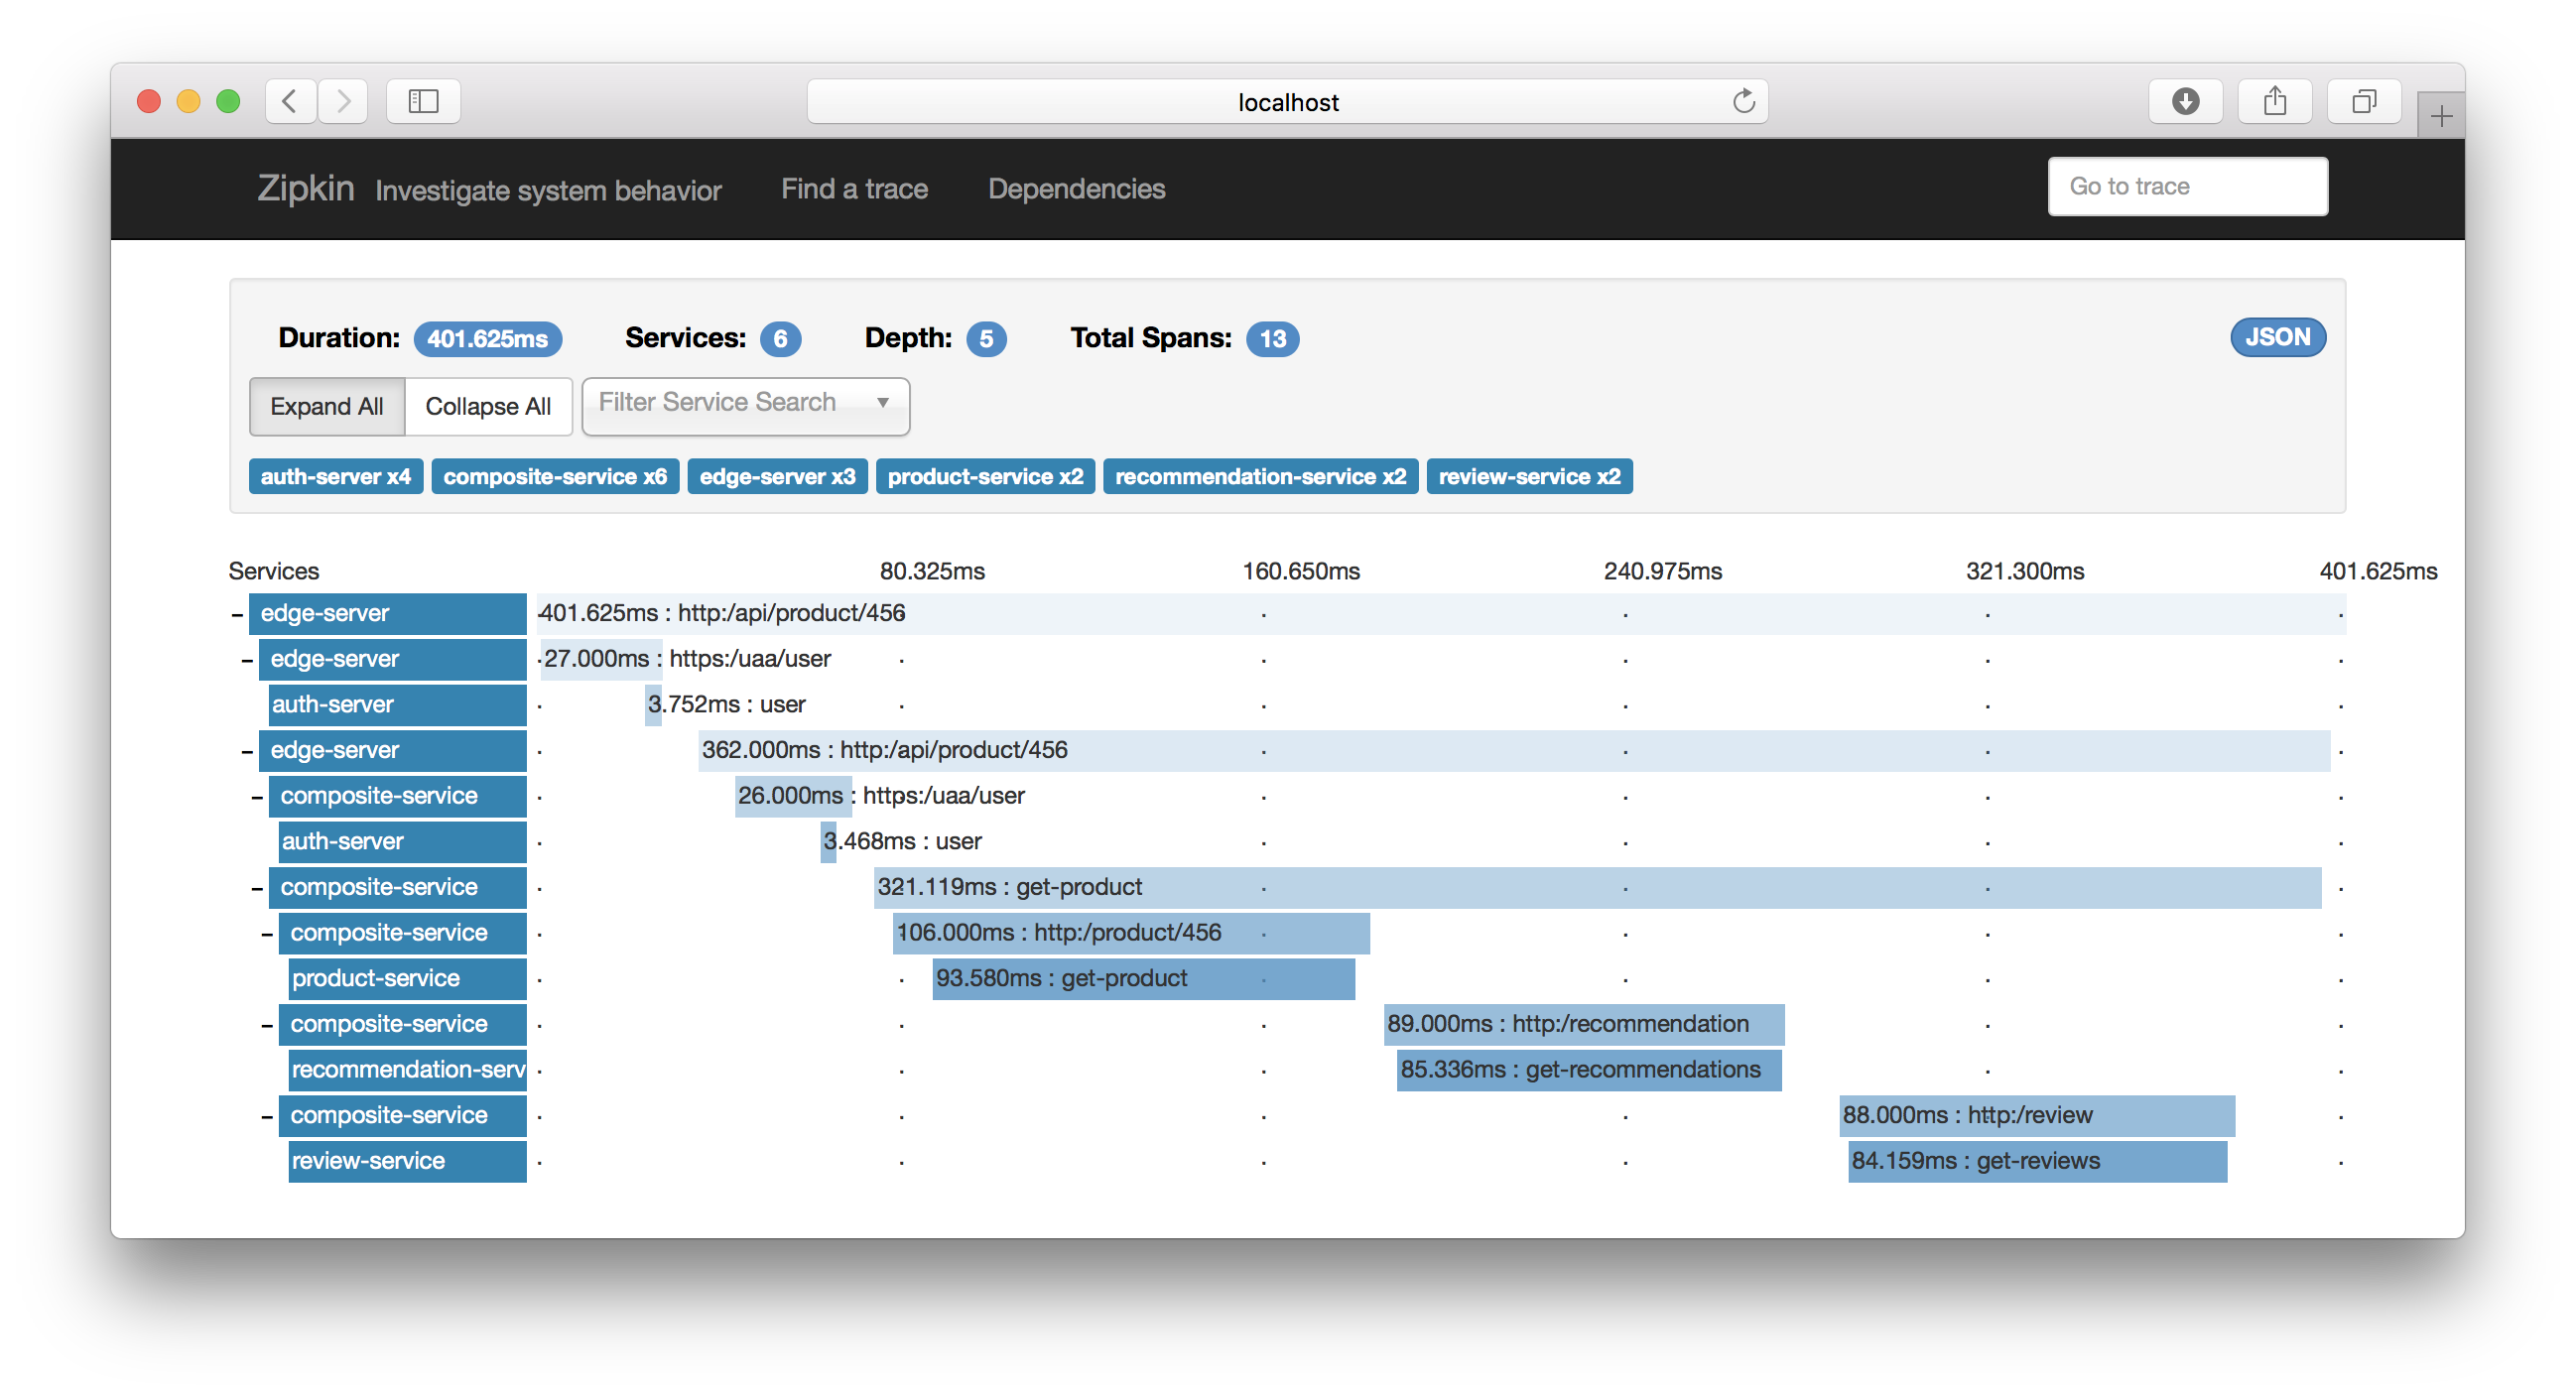
\includegraphics[scale=0.16]{pictures/zipkin-sample.png}
		\end{center}
		\legend{Fonte: \url{http://callistaenterprise.se/assets/blogg/build-microservices-part-7/Zipkin-sample.png}}
	\end{figure}
	
	\begin{figure}[htb]
		\caption{\label{fig_topology_map}Exemplo de Mapa de Topologia de Serviços}
		\begin{center}
		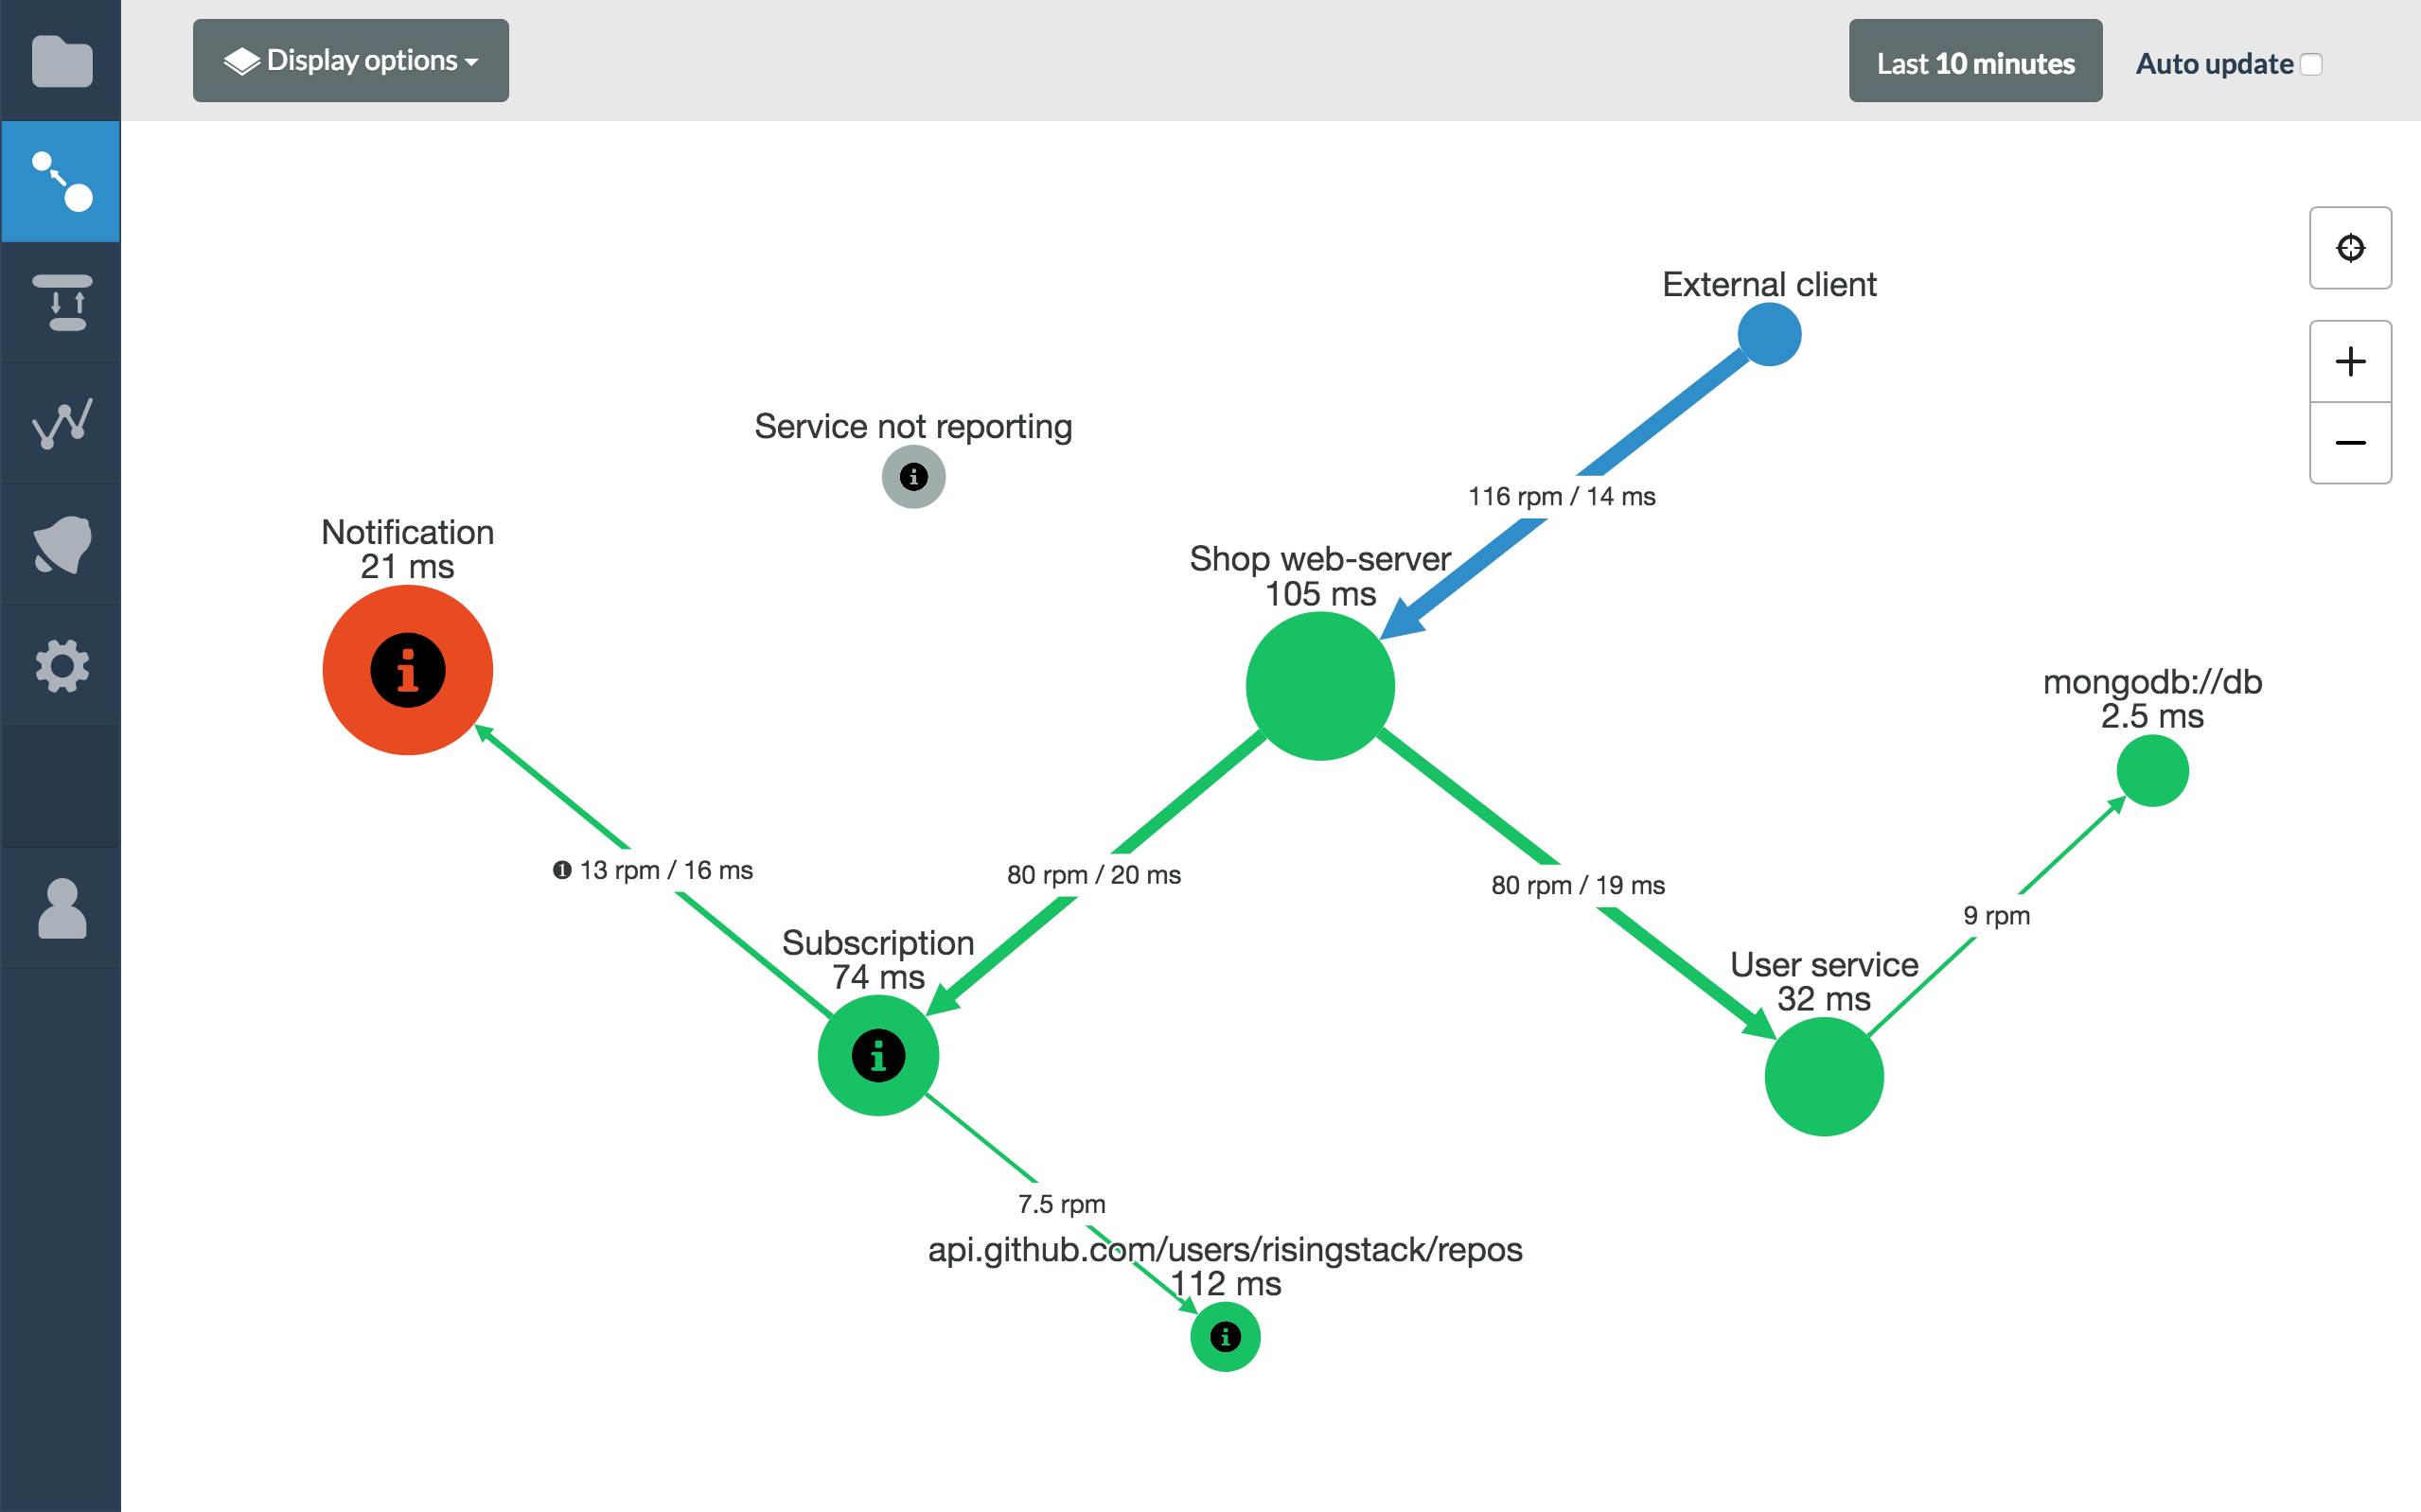
\includegraphics[scale=0.16]{pictures/service_topology_map.png}
		\end{center}
		\legend{Fonte: \url{https://blog-assets.risingstack.com/2016/May/Distributed_transaction_tracing_with_service_topology_map_trace_by_risingstack-1462456507669.png}}
	\end{figure}
	
	\subsection{OpenTracing}
	
	Nessa seção iremos entender um pouco melhor como se organiza e os principais conceitos estabelecidos pelo padrão OpenTracing. Entre eles vamos entender como é feita a correlação entre eventos enviados pelos serviços e quais os mecanismos padrões utilizados para que isso seja efetivamente realizado por aplicações reais.
	
	